% Compatibility shims for a newer local hyperref with the installed LaTeX kernel.
\providecommand\IfDocumentMetadataT[1]{}
\providecommand\IfDocumentMetadataTF[2]{#2}
\documentclass[aspectratio=169,9pt]{beamer}
\NeedsTeXFormat{LaTeX2e}
% Shared Agrawal homework style (loaded with \input from either deck).

\RequirePackage{fontspec}
\RequirePackage{amsmath,amssymb,mathtools}
\RequirePackage{booktabs}
\RequirePackage{graphicx}
\RequirePackage{microtype}
\RequirePackage{ragged2e}
\RequirePackage{hyperref}
\RequirePackage{tikz}
\usetikzlibrary{positioning}

\IfFontExistsTF{Avenir Next}{\setsansfont{Avenir Next}}{\setsansfont{TeX Gyre Heros}}

% Palette sampled from the supplied reference screenshot.
\definecolor{AgNavy}{HTML}{0C2852}
\definecolor{AgRed}{HTML}{982A34}
\definecolor{AgGraphite}{HTML}{000000}
\definecolor{AgMuted}{HTML}{000000}
\definecolor{AgRedTitle}{HTML}{F4E8EA}
\definecolor{AgRedBody}{HTML}{F9F5F5}
\definecolor{AgBlueTitle}{HTML}{EBEEF1}
\definecolor{AgBlueBody}{HTML}{F5F6F8}
\definecolor{AgDivider}{HTML}{D9DEE4}

\usetheme{default}
\usefonttheme{professionalfonts}
\setbeamertemplate{navigation symbols}{}
\setbeamersize{text margin left=0.85cm,text margin right=0.85cm}

\setbeamercolor{background canvas}{bg=white}
\setbeamercolor{normal text}{fg=AgGraphite,bg=white}
\setbeamercolor{frametitle}{fg=white,bg=AgNavy}
\setbeamercolor{structure}{fg=AgNavy}
\setbeamercolor{alerted text}{fg=AgRed}
\setbeamercolor{ag red title}{fg=AgRed,bg=AgRedTitle}
\setbeamercolor{ag red body}{fg=AgGraphite,bg=AgRedBody}
\setbeamercolor{ag blue title}{fg=AgNavy,bg=AgBlueTitle}
\setbeamercolor{ag blue body}{fg=AgGraphite,bg=AgBlueBody}
\setbeamercolor{ag accent line}{bg=AgRed}
\setbeamercolor{ag divider line}{bg=AgDivider}

\setbeamerfont{frametitle}{size=\large,series=\bfseries}
\setbeamerfont{normal text}{size=\normalsize}
\setbeamerfont{block title}{size=\normalsize,series=\bfseries}
\setbeamerfont{footline}{size=\scriptsize}

\setbeamertemplate{frametitle}{%
  \nointerlineskip
  \begin{beamercolorbox}[wd=\paperwidth,ht=0.62cm,dp=0.23cm,leftskip=0.40cm]{frametitle}%
    \usebeamerfont{frametitle}\insertframetitle
  \end{beamercolorbox}%
  \nointerlineskip
  \hbox{%
    \begin{beamercolorbox}[wd=1.05cm,ht=0.018cm,dp=0cm]{ag accent line}\end{beamercolorbox}%
    \begin{beamercolorbox}[wd=\dimexpr\paperwidth-1.05cm\relax,ht=0.018cm,dp=0cm]{ag divider line}\end{beamercolorbox}%
  }%
}

\setbeamertemplate{footline}{}

\setbeamertemplate{itemize item}{\color{AgNavy}\raise0.12ex\hbox{\scriptsize$\blacktriangleright$}}
\setbeamertemplate{itemize subitem}{\color{AgRed}\raise0.08ex\hbox{\tiny$\bullet$}}
\setlength{\leftmargini}{1.05em}
\setlength{\leftmarginii}{1.0em}

\newcommand{\E}{\mathbb{E}}
\newcommand{\Var}{\operatorname{Var}}
\newcommand{\Cov}{\operatorname{Cov}}

\newcommand{\agredblock}[2]{%
  \begin{beamercolorbox}[wd=\linewidth,sep=0.11cm]{ag red title}\usebeamerfont{block title}#1\end{beamercolorbox}%
  \nointerlineskip
  \begin{beamercolorbox}[wd=\linewidth,sep=0.14cm]{ag red body}#2\end{beamercolorbox}%
}

\newcommand{\agblueblock}[2]{%
  \begin{beamercolorbox}[wd=\linewidth,sep=0.11cm]{ag blue title}\usebeamerfont{block title}#1\end{beamercolorbox}%
  \nointerlineskip
  \begin{beamercolorbox}[wd=\linewidth,sep=0.14cm]{ag blue body}#2\end{beamercolorbox}%
}

\newcommand{\agcompactredblock}[2]{%
  \begin{beamercolorbox}[wd=\linewidth,sep=0.08cm]{ag red title}\usebeamerfont{block title}#1\end{beamercolorbox}%
  \nointerlineskip
  \begin{beamercolorbox}[wd=\linewidth,sep=0.09cm]{ag red body}#2\end{beamercolorbox}%
}

\newcommand{\agcompactblueblock}[2]{%
  \begin{beamercolorbox}[wd=\linewidth,sep=0.08cm]{ag blue title}\usebeamerfont{block title}#1\end{beamercolorbox}%
  \nointerlineskip
  \begin{beamercolorbox}[wd=\linewidth,sep=0.09cm]{ag blue body}#2\end{beamercolorbox}%
}

% Roomier variants used by the short deck: wider internal gutters without
% changing the more compact geometry of the 26-frame presentation.
\newcommand{\agshortredblock}[2]{%
  \begin{beamercolorbox}[wd=\linewidth,sep=0.12cm,leftskip=0.08cm,rightskip=0.08cm]{ag red title}\usebeamerfont{block title}#1\end{beamercolorbox}%
  \nointerlineskip
  \begin{beamercolorbox}[wd=\linewidth,sep=0.16cm,leftskip=0.10cm,rightskip=0.10cm]{ag red body}#2\end{beamercolorbox}%
}

\newcommand{\agshortblueblock}[2]{%
  \begin{beamercolorbox}[wd=\linewidth,sep=0.12cm,leftskip=0.08cm,rightskip=0.08cm]{ag blue title}\usebeamerfont{block title}#1\end{beamercolorbox}%
  \nointerlineskip
  \begin{beamercolorbox}[wd=\linewidth,sep=0.16cm,leftskip=0.10cm,rightskip=0.10cm]{ag blue body}#2\end{beamercolorbox}%
}

\newcommand{\agshortcompactredblock}[2]{%
  \begin{beamercolorbox}[wd=\linewidth,sep=0.10cm,leftskip=0.08cm,rightskip=0.08cm]{ag red title}\usebeamerfont{block title}#1\end{beamercolorbox}%
  \nointerlineskip
  \begin{beamercolorbox}[wd=\linewidth,sep=0.12cm,leftskip=0.12cm,rightskip=0.12cm]{ag red body}#2\end{beamercolorbox}%
}

\newcommand{\agshortcompactblueblock}[2]{%
  \begin{beamercolorbox}[wd=\linewidth,sep=0.10cm,leftskip=0.08cm,rightskip=0.08cm]{ag blue title}\usebeamerfont{block title}#1\end{beamercolorbox}%
  \nointerlineskip
  \begin{beamercolorbox}[wd=\linewidth,sep=0.12cm,leftskip=0.12cm,rightskip=0.12cm]{ag blue body}#2\end{beamercolorbox}%
}

\newcommand{\agshorttwocol}[4]{%
  \noindent\hspace*{0.18cm}%
  \begin{minipage}[t]{#1\linewidth}\vspace{0pt}#2\end{minipage}%
  \hfill
  \begin{minipage}[t]{#3\linewidth}\vspace{0pt}#4\end{minipage}%
  \hspace*{0.18cm}\par
}

\newcommand{\agtitlepage}[3]{%
  \setbeamertemplate{footline}{}%
  \vspace*{1.68cm}
  {\fontsize{17}{20}\selectfont\bfseries The Economics of Bicycles for the Mind\par}
  \vspace{0.18cm}
  {\fontsize{12.5}{15}\selectfont #1\par}
  \vspace{0.48cm}
  {\color{AgRed}\rule{\linewidth}{0.48pt}}
  \vspace{0.55cm}
  {\normalsize\bfseries Gabriel Saco\par}
  \vspace{0.06cm}
  {\normalsize August 24, 2026\par}
  \vspace{0.22cm}
  {\small Universidad del Pac\'ifico\par}
  \vspace{0.22cm}
  {\small\color{AgMuted}Agrawal, Gans \& Goldfarb (2025) \textperiodcentered\ NBER WP 34034\par}
  \vspace{0.12cm}
  {\small\href{https://github.com/gsaco/ai-02-agrawal}{\color{AgNavy}\ttfamily github.com/gsaco/ai-02-agrawal}\par}
  \vfill
  {\scriptsize\color{AgMuted}#2\hfill #3\par}
}

\newcommand{\agrestorefootline}{%
  \setbeamertemplate{footline}{}%
}


\begin{document}

% 1
\begin{frame}[plain]
  \agtitlepage
    {Cognitive tools, human judgment, and inequality}
    {Extended technical presentation}
    {}
\end{frame}
\agrestorefootline

% 2
\begin{frame}[t]{Roadmap: model, propositions, and audit}
  \vspace{0.50cm}
  \begin{columns}[T,onlytextwidth]
    \begin{column}{0.31\textwidth}
      \agredblock{1. Mechanism}{%
        \small A cognitive tool raises direct performance but lowers the marginal
        return to implementation effort.
      }
    \end{column}
    \begin{column}{0.31\textwidth}
      \agblueblock{2. Propositions}{%
        \small Less effort, more value; adoption depends differently on skill and
        two forms of judgment.
      }
    \end{column}
    \begin{column}{0.31\textwidth}
      \agredblock{3. Inequality audit}{%
        \small Identify the variance object, derive its threshold, and check the
        paper's endpoint claim.
      }
    \end{column}
  \end{columns}
  \vspace{0.48cm}
  \agblueblock{Contribution of this repository}{%
    \small A symbolic derivation, an exact-moment counterexample, a separate
    individual-benefit calculation, and a documented interior-domain audit.
  }
\end{frame}

% 3
\begin{frame}[t]{Motivating example I: computer-aided design}
  \vspace{0.50cm}
  \begin{columns}[T,onlytextwidth]
    \begin{column}{0.45\textwidth}
      \agredblock{Without the tool}{%
        \small The worker calculates and draws manually. Each improvement uses
        implementation effort $e$, transformed by skill $s$ into output $v(se)$.
      }
      \vspace{0.28cm}
      \[
        M(e)=v(se)-c(e),
      \]
      \[
        v'(se^*)s=c'(e^*).
      \]
    \end{column}
    \begin{column}{0.08\textwidth}
      \centering\vspace{1.4cm}{\color{AgRed}\Large$\Longrightarrow$}
    \end{column}
    \begin{column}{0.45\textwidth}
      \agblueblock{With the tool}{%
        \small Software implements calculations and visualizations more easily.
        Direct task value rises while additional human effort becomes less useful.
      }
      \vspace{0.28cm}
      \[
        e^*(1)<e^*(0),
      \]
      \[
        M(e^*(1);1)>M(e^*(0);0).
      \]
    \end{column}
  \end{columns}
  \vfill
  {\small\color{AgMuted}Computer assistance is the paper's clean example of “more output with less input.”}
\end{frame}

% 4
\begin{frame}[t]{Motivating example II: AI-assisted prediction}
  \vspace{0.42cm}
  \agblueblock{Diagnosis separates prediction from judgment}{%
    \small Effort and implementation skill improve diagnostic accuracy $p(se)$.
    Payoff judgment $\alpha$ is the ability to select and apply the right treatment
    after receiving a signal.
  }
  \vspace{0.34cm}
  \begin{columns}[T,onlytextwidth]
    \begin{column}{0.50\textwidth}
      \textbf{Objective}
      \[
        \max_{e\ge0}\ \alpha\{p(se)\Delta_{C}+[1-p(se)]\Delta_{W}\}-c(e).
      \]
      \small AI shifts accuracy from $p(se)$ to $p(se+\theta)$.
    \end{column}
    \begin{column}{0.46\textwidth}
      \textbf{Economic separation}
      \begin{itemize}\small
        \item Better prediction is valuable only when the decision-maker can act.
        \item Endogenous effort may fall after tool adoption.
        \item Payoff judgment complements the tool only if realized accuracy rises.
      \end{itemize}
    \end{column}
  \end{columns}
\end{frame}

% 5
\begin{frame}[t]{The task-improvement process}
  \vspace{0.55cm}
  \centering
  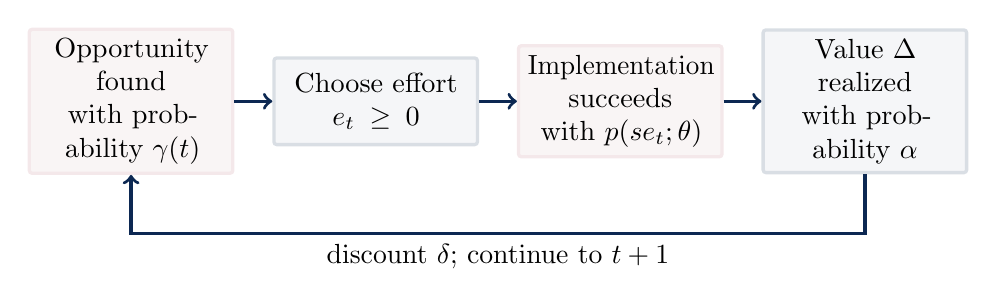
\begin{tikzpicture}[
    node distance=0.48cm,
    box/.style={draw=AgDivider,very thick,rounded corners=1pt,minimum height=1.10cm,text width=2.35cm,align=center,fill=AgBlueBody},
    redbox/.style={box,fill=AgRedBody,draw=AgRedTitle},
    arrow/.style={->,very thick,draw=AgNavy}
  ]
    \node[redbox] (opp) {Opportunity found\\with probability $\gamma(t)$};
    \node[box,right=of opp] (effort) {Choose effort\\$e_t\ge0$};
    \node[redbox,right=of effort] (success) {Implementation succeeds\\with $p(se_t;\theta)$};
    \node[box,right=of success] (payoff) {Value $\Delta$ realized\\with probability $\alpha$};
    \draw[arrow] (opp) -- (effort);
    \draw[arrow] (effort) -- (success);
    \draw[arrow] (success) -- (payoff);
    \draw[arrow] (payoff.south) |- ++(0,-0.75) -| node[pos=.25,below,align=center]{discount $\delta$; continue to $t+1$} (opp.south);
  \end{tikzpicture}
  \par
  \vspace{0.55cm}
  \agblueblock{Stopping rule}{%
    \small If no new opportunity is perceived, the process ends. Conditional on
    an opportunity, the effort problem is identical in every round.
  }
\end{frame}

% 6
\begin{frame}[t]{Three human capabilities}
  \vspace{0.48cm}
  \begin{columns}[T,onlytextwidth]
    \begin{column}{0.31\textwidth}
      \agblueblock{Implementation skill $s$}{%
        \small How effectively effort becomes a successful implementation.
        It enters through $se_t$.
      }
    \end{column}
    \begin{column}{0.31\textwidth}
      \agredblock{Payoff judgment $\alpha$}{%
        \small The probability of recognizing and extracting value from a
        successful implementation.
      }
    \end{column}
    \begin{column}{0.31\textwidth}
      \agblueblock{Opportunity judgment $\gamma(t)$}{%
        \small The probability of finding another opportunity to improve the
        task in round $t$.
      }
    \end{column}
  \end{columns}
  \vspace{0.50cm}
  \agredblock{Why the decomposition matters}{%
    \small A tool can substitute for implementation skill while amplifying the
    value of judgment. Treating all three as a single “skill” would hide the
    distributional mechanism.
  }
\end{frame}

% 7
\begin{frame}[t]{General optimization problem}
  \vspace{0.42cm}
  \begin{columns}[T,onlytextwidth]
    \begin{column}{0.53\textwidth}
      \agblueblock{Per opportunity}{%
        \small
        \[
          e_t^*(\theta)\in\arg\max_{e_t\ge0}
          \{p(se_t;\theta)\alpha\Delta-c(e_t;\theta)\}.
        \]
        Interior FOC:
        \[
          p'(se_t^*;\theta)s\alpha\Delta=c'(e_t^*;\theta).
        \]
      }
    \end{column}
    \begin{column}{0.44\textwidth}
      \agredblock{Across opportunities}{%
        \small
        \[
          V_0(\theta)=\sum_{t=0}^{\infty}
          \left(\prod_{i=0}^{t}\gamma(i)\right)
          \delta^tM(e_t^*(\theta);\theta).
        \]
        The opportunity path scales value, but it does not change the
        conditional effort problem.
      }
    \end{column}
  \end{columns}
\end{frame}

% 8
\begin{frame}[t]{Definition 1: what counts as a cognitive tool?}
  \vspace{0.42cm}
  \agredblock{Direct effects}{%
    \small For every $e$ and $\theta'>\theta$,
    \[
      p(se;\theta')\ge p(se;\theta),
      \qquad c(e;\theta')\le c(e;\theta),
    \]
    with a strict improvement somewhere relevant for a strict value gain.
  }
  \vspace{0.32cm}
  \agblueblock{Marginal substitution}{%
    \small For $e>0$,
    \[
      \frac{p'(se;\theta')}{c'(e;\theta')}
      <\frac{p'(se;\theta)}{c'(e;\theta)}.
    \]
    Higher tool quality reduces the marginal success obtained per unit of
    marginal human effort cost.
  }
\end{frame}

% 9
\begin{frame}[t]{Proposition 1: more value with less effort}
  \vspace{0.48cm}
  \agredblock{Statement}{%
    \small As tool quality moves from $\theta=0$ to $\theta=1$,
    \[
      e_t^*(1)<e_t^*(0)\ \forall t,
      \qquad e_t^*(\theta)=e^*(\theta)\ \forall t,
      \qquad V_0(1)>V_0(0).
    \]
  }
  \vspace{0.40cm}
  \agblueblock{Conditions carried by the result}{%
    \small A well-defined selected optimum; the cognitive-tool inequalities;
    positive $s\alpha\Delta$ and finite discounted opportunities; and interior
    optima or the corresponding strict Kuhn--Tucker comparison at the boundary.
  }
  \vfill
  {\small\color{AgMuted}The time-invariance result comes from repeating the same conditional problem, not from constant opportunity arrival.}
\end{frame}

% 10
\begin{frame}[t]{Proposition 1: proof logic and economics}
  \vspace{0.42cm}
  \begin{columns}[T,onlytextwidth]
    \begin{column}{0.48\textwidth}
      \agblueblock{Effort comparison}{%
        \small The FOC equates $s\alpha\Delta\,p'/c'$ to one. Definition 1 shifts
        this ratio downward at every positive effort, so the new optimum moves
        to a lower $e$ under the paper's monotonicity logic.
      }
    \end{column}
    \begin{column}{0.48\textwidth}
      \agredblock{Value comparison}{%
        \small At the old effort, the tool weakly raises success and weakly lowers
        cost. Re-optimizing cannot reduce that improved payoff:
        \[
          M(e^*(1);1)>M(e^*(0);0).
        \]
      }
    \end{column}
  \end{columns}
  \vspace{0.46cm}
  \agblueblock{Economic intuition}{%
    \small The tool handles the low-hanging implementation work. Human effort
    falls, but optimized net task value rises because the entire opportunity
    payoff schedule has improved.
  }
\end{frame}

% 11
\begin{frame}[t]{Adoption value and the opportunity multiplier}
  \vspace{0.48cm}
  \agblueblock{Factorization}{%
    \small Define
    \[
      \Gamma=\sum_{t=0}^{\infty}
      \left(\prod_{i=0}^{t}\gamma(i)\right)\delta^t.
    \]
    Since optimal effort is time-invariant,
    \[
      V_0(1)-V_0(0)
      =\Gamma\,[M(e^*(1);1)-M(e^*(0);0)]>0.
    \]
  }
  \vspace{0.38cm}
  \agredblock{Interpretation}{%
    \small Adoption value equals a per-opportunity productivity gain multiplied
    by the discounted number and timing of opportunities on which the tool can be used.
  }
\end{frame}

% 12
\begin{frame}[t]{Proposition 2.1: opportunity judgment}
  \vspace{0.48cm}
  \begin{columns}[T,onlytextwidth]
    \begin{column}{0.48\textwidth}
      \agredblock{General sequence}{%
        \small Every component $\gamma(t)$ affects the probability of reaching
        all later opportunities. Hence better opportunity judgment raises
        adoption value whenever the per-opportunity gain is positive.
      }
    \end{column}
    \begin{column}{0.48\textwidth}
      \agblueblock{Geometric special case}{%
        \small If $\gamma(0)=\gamma_0$ and $\gamma(t)=\gamma$ for $t>0$,
        \[
          \Gamma=\frac{\gamma_0}{1-\delta\gamma},
          \qquad \delta\gamma<1.
        \]
      }
    \end{column}
  \end{columns}
  \vspace{0.46cm}
  \agredblock{Mechanism}{%
    \small Opportunity judgment does not make implementation better at one
    opportunity; it increases how often the agent can apply the tool's gain.
  }
\end{frame}

% 13
\begin{frame}[t]{Proposition 2.2: payoff judgment}
  \vspace{0.48cm}
  \agblueblock{Envelope calculation}{%
    \small
    \[
      \frac{\partial[V_0(1)-V_0(0)]}{\partial\alpha}
      =\Gamma\Delta\,[p(se^*(1);1)-p(se^*(0);0)].
    \]
  }
  \vspace{0.38cm}
  \begin{columns}[T,onlytextwidth]
    \begin{column}{0.48\textwidth}
      \agredblock{Complementarity}{%
        \small Payoff judgment raises adoption value if realized implementation
        success is weakly higher with the tool.
      }
    \end{column}
    \begin{column}{0.48\textwidth}
      \agblueblock{Why the sign is ambiguous}{%
        \small The direct tool effect raises success, but endogenous effort falls.
        Definition 1 alone does not determine which force dominates.
      }
    \end{column}
  \end{columns}
\end{frame}

% 14
\begin{frame}[t]{Proposition 2.3: implementation skill}
  \vspace{0.42cm}
  \agredblock{Optimizer-level derivative}{%
    \small
    \[
      \frac{\partial[V_0(1)-V_0(0)]}{\partial s}
      =\Gamma\alpha\Delta
      \{p_s(se^*(1);1)-p_s(se^*(0);0)\}.
    \]
  }
  \vspace{0.34cm}
  \agblueblock{Paper's condition and the caveat}{%
    \small The paper invokes $p_{s\theta}<0$ to call tool quality and skill
    substitutes. But that cross-partial holds effort fixed, whereas the displayed
    derivative compares two different optimal efforts. An additional restriction
    is required to sign the optimizer-level bracket in full generality.
  }
  \vfill
  {\small\color{AgMuted}The intended mechanism remains inverse skill bias: lower-skill workers receive the larger marginal tool boost.}
\end{frame}

% 15
\begin{frame}[t]{Proposition 2.4: early versus late opportunities}
  \vspace{0.42cm}
  \agblueblock{Correct derivative for a general path}{%
    \small
    \[
      \frac{\partial\Gamma}{\partial\gamma(t)}
      =\sum_{k=t}^{\infty}\delta^k
      \prod_{\substack{i=0\\i\ne t}}^{k}\gamma(i).
    \]
    Changing $\gamma(t)$ affects the chance of reaching every subsequent $k\ge t$.
  }
  \vspace{0.34cm}
  \agredblock{Audit of the displayed proposition}{%
    \small Proposition 2's ratio keeps only the first $k=t$ product. The general
    ranking therefore depends on the whole opportunity path. Earlier opportunities
    do receive greater weight in the geometric special case under discounting.
  }
\end{frame}

% 16
\begin{frame}[t]{Inequality specialization: all maintained assumptions}
  \vspace{0.34cm}
  \begin{columns}[T,onlytextwidth]
    \begin{column}{0.48\textwidth}
      \agblueblock{Functional form}{%
        \small
        \[
          p(se;\theta)=\sqrt{se+\theta},\qquad c(e)=e.
        \]
        $\gamma(0)=\gamma_0$, $\gamma(t)=\gamma$ for $t>0$, and
        $\delta\gamma<1$.
      }
      \vspace{0.26cm}
      \agredblock{Tool quality}{%
        \small $\theta\in[0,\infty)$ is treated as continuous, even though the
        earlier adoption comparison used $\theta\in\{0,1\}$.
      }
    \end{column}
    \begin{column}{0.48\textwidth}
      \agredblock{Heterogeneity}{%
        \small $\alpha,\gamma_0,\gamma,s$ are independent, have positive support,
        means $\mu_i$, variances $\sigma_i^2$, and satisfy the paper's
        $\mu_i>3\sigma_i$ restriction.
      }
      \vspace{0.26cm}
      \agblueblock{Interiority}{%
        \small The closed form applies only where every worker satisfies
        \[
          \theta<\alpha^2\Delta^2s^2/4.
        \]
      }
    \end{column}
  \end{columns}
\end{frame}

% 17
\begin{frame}[t]{Closed form: effort, net benefit, and value}
  \vspace{0.42cm}
  \agblueblock{Solve the FOC}{%
    \small
    \[
      \frac{\alpha\Delta s}{2\sqrt{se^*(\theta)+\theta}}=1
      \quad\Longrightarrow\quad
      e^*(\theta)=\frac{\alpha^2\Delta^2s}{4}-\frac{\theta}{s}.
    \]
  }
  \vspace{0.30cm}
  \begin{columns}[T,onlytextwidth]
    \begin{column}{0.48\textwidth}
      \agredblock{Per opportunity}{%
        \small
        \[
          M(\theta)=\frac{\alpha^2\Delta^2s}{4}+\frac{\theta}{s}.
        \]
        Tool quality has an inverse-skill boost $\theta/s$.
      }
    \end{column}
    \begin{column}{0.48\textwidth}
      \agblueblock{Continuation value}{%
        \small
        \[
          V(\theta)=\Gamma\left(\frac{\alpha^2\Delta^2s}{4}+\frac{\theta}{s}\right).
        \]
        Opportunity judgment multiplies both components.
      }
    \end{column}
  \end{columns}
\end{frame}

% 18
\begin{frame}[t]{Proposition 3: corrected exact statement}
  \vspace{0.34cm}
  \agcompactblueblock{Mean}{%
    \small
    \[
      \frac{d\E[V(\theta)]}{d\theta}=\E[\Gamma]\E[1/s]>0.
    \]
  }
  \vspace{0.15cm}
  \agcompactredblock{Variance}{%
    \small If
    \[
      \frac{\E[\Gamma^2]}{\E[\Gamma]^2}<\mu_s\E[1/s]
      \quad\text{and}\quad \Var(\Gamma/s)>0,
    \]
    then the interior $\Var[V(\theta)]$ is strictly convex, decreases before
    $\theta^*$, and increases after $\theta^*$.
  }
  \vspace{0.15cm}
  \agcompactblueblock{Endpoint}{%
    \small The printed claim of a positive slope at $\theta=1$ additionally
    requires $\theta^*<1$ and an interior solution there.
  }
\end{frame}

% 19
\begin{frame}[t]{Mean effect: productivity always rises}
  \vspace{0.48cm}
  \agblueblock{Expectation}{%
    \small Independence implies
    \[
      \E[V(\theta)]
      =\E[\Gamma]\left\{
      \frac{\Delta^2}{4}\E[\alpha^2]\mu_s
      +\theta\E[1/s]\right\}.
    \]
  }
  \vspace{0.36cm}
  \agredblock{Comparative static}{%
    \small
    \[
      \frac{d\E[V(\theta)]}{d\theta}
      =\E[\Gamma]\E[1/s]>0.
    \]
    Every worker's interior tool boost is positive, and averaging preserves the sign.
  }
  \vfill
  {\small\color{AgMuted}The controversy is about dispersion, not the sign of mean productivity.}
\end{frame}

% 20
\begin{frame}[t]{Variance algebra I: separate multiplier and payoff}
  \vspace{0.40cm}
  \agblueblock{Product variance}{%
    \small Since $\Gamma$ and $M(\theta)$ are independent,
    \[
      \Var[V(\theta)]
      =\E[\Gamma^2]\Var[M(\theta)]
      +\Var(\Gamma)\E[M(\theta)]^2.
    \]
  }
  \vspace{0.28cm}
  \agredblock{Quadratic per-opportunity variance}{%
    \small With $K=\Delta^2/4$,
    \[
      \E[M]=K\E[\alpha^2]\mu_s+\theta\E[1/s],
      \qquad \Var(M)=A+B\theta+C\theta^2,
    \]
    where $B=2K\E[\alpha^2]\{1-\mu_s\E[1/s]\}\le0$ and
    $C=\Var(1/s)\ge0$.
  }
\end{frame}

% 21
\begin{frame}[t]{Variance algebra II: derivative and threshold}
  \vspace{0.36cm}
  \agredblock{Linear slope}{%
    \small Collecting the derivative gives
    \[
      \frac{d\Var[V(\theta)]}{d\theta}
      =a_0+2\theta\Var(\Gamma/s),
    \]
    \[
      a_0=\frac{\Delta^2\E[\alpha^2]}{2}
      \{\E[\Gamma^2]-\E[\Gamma]^2\mu_s\E[1/s]\}.
    \]
  }
  \vspace{0.25cm}
  \agblueblock{Condition (30)}{%
    \small
    \[
      \frac{\E[\Gamma^2]}{\E[\Gamma]^2}<\mu_s\E[1/s]
      \quad\Longleftrightarrow\quad a_0<0.
    \]
    It is precisely the condition for an initially negative variance slope.
  }
\end{frame}

% 22
\begin{frame}[t]{Turning point: what the U-shape really says}
  \vspace{0.42cm}
  \begin{columns}[T,onlytextwidth]
    \begin{column}{0.48\textwidth}
      \agblueblock{Unique interior minimum}{%
        \small If $\Var(\Gamma/s)>0$,
        \[
          \theta^*=-\frac{a_0}{2\Var(\Gamma/s)}>0,
        \]
        with a negative slope below $\theta^*$ and a positive slope above it.
      }
    \end{column}
    \begin{column}{0.48\textwidth}
      \agredblock{Two competing forces}{%
        \small
        \textbf{Inverse skill bias:} $\theta/s$ helps low-$s$ workers more.\\[0.12cm]
        \textbf{Judgment amplification:} heterogeneous $\Gamma$ magnifies who can
        use that boost repeatedly.
      }
    \end{column}
  \end{columns}
  \vspace{0.45cm}
  \agblueblock{Correct scope}{%
    \small This is a result for the cross section and for the common interior
    tool-quality range. It is not a global claim over $\theta\in[0,\infty)$.
  }
\end{frame}

% 23
\begin{frame}[t]{The professor's three questions, answered}
  \vspace{0.40cm}
  \agcompactredblock{1. Variance of what, with respect to what?}{%
    \small Cross-sectional variance of continuation value $V_i(\theta)$,
    interpreted as wages, as continuous tool quality $\theta$ changes.
  }
  \vspace{0.18cm}
  \agcompactblueblock{2. Is the result unconditional?}{%
    \small No. It needs the specialized functional form, independence and
    support restrictions, $\delta\gamma<1$, condition (30),
    $\Var(\Gamma/s)>0$, and a common interior range.
  }
  \vspace{0.18cm}
  \agcompactredblock{3. What about individual benefit?}{%
    \small
    \[
      D_i(\theta)=\theta\Gamma_i/s_i,
      \qquad \Var[D(\theta)]=\theta^2\Var(\Gamma/s),
    \]
    so benefit variance rises monotonically for $\theta>0$.
  }
\end{frame}

% 24
\begin{frame}[t]{Internal slips and proof gaps}
  \vspace{0.34cm}
  \begin{columns}[T,onlytextwidth]
    \begin{column}{0.48\textwidth}
      \agredblock{Variance section}{%
        \small
        \begin{itemize}
          \item Equation (32) needs $\theta^*<1$ for its slope-at-one claim.
          \item The printed $\Delta>2/(s\sqrt\alpha)$ does not ensure $e^*(1)>0$;
          the algebra requires $\Delta>2/(\alpha s)$.
          \item That corrected interior condition forces $p^*(1)>1$, conflicting
          with the general model's probability bound.
        \end{itemize}
      }
    \end{column}
    \begin{column}{0.48\textwidth}
      \agblueblock{Proposition 2}{%
        \small
        \begin{itemize}
          \item The displayed general timing ratio omits all future terms
          affected by $\gamma(t)$.
          \item $p_{s\theta}<0$ holds effort fixed and does not alone sign the
          comparison across two endogenous effort choices.
        \end{itemize}
      }
    \end{column}
  \end{columns}
  \vfill
  {\small\color{AgMuted}These points qualify particular claims; they do not erase the model's central substitution mechanism.}
\end{frame}

% 25
\begin{frame}[t]{Exact-moment counterexample and SymPy audit}
  \vspace{0.42cm}
  \agblueblock{Independent-uniform construction}{%
    \small All variables are mutually independent, with
    \[
      \alpha\in[.75,.85],\qquad \gamma_0\in[.48,.52],\qquad
      \gamma\in[.36,.44],\qquad s\in[.8,1],
    \]
    and $\delta=.8$, $\Delta=5$. Their supports are positive and each satisfies
    $\mu_i>3\sigma_i$.
  }
  \vspace{0.28cm}
  \agredblock{Exact symbolic and moment checks}{%
    \small
    \[
      \frac{\E[\Gamma^2]}{\E[\Gamma]^2}=1.0012732
      <1.0041460=\mu_s\E[1/s],
      \qquad \theta^*=1.7007141,
    \]
    \[
      \left.\frac{d\Var[V(\theta)]}{d\theta}\right|_{\theta=1}
      =-0.0051337<0,
      \qquad \min_i\frac{\alpha_i^2\Delta^2s_i^2}{4}=2.25.
    \]
  }
  \vspace{0.28cm}
  \agblueblock{What the counterexample establishes}{%
    \small Condition (30) holds and the turning point lies in the common interior
    range, yet the variance slope is still negative at $\theta=1$. Thus the
    paper's endpoint claim needs the missing condition $\theta^*<1$.
  }
\end{frame}

% 26
\begin{frame}[t]{Limiting cases and final takeaways}
  \vspace{0.34cm}
  \begin{columns}[T,onlytextwidth]
    \begin{column}{0.48\textwidth}
      \agblueblock{Limiting cases}{%
        \small
        \begin{itemize}
          \item Constant $\Gamma$: skill heterogeneity can generate the initial compression.
          \item Constant $s$: the equalizing inverse-skill channel disappears.
          \item Constant $\Gamma/s$: no strict quadratic curvature.
          \item Large $\theta$: workers hit $e=0$ at heterogeneous thresholds.
        \end{itemize}
      }
    \end{column}
    \begin{column}{0.48\textwidth}
      \agredblock{Three takeaways}{%
        \small
        \begin{enumerate}
          \item Cognitive tools can raise value while reducing human effort.
          \item Skill and two forms of judgment have different adoption returns.
          \item The U-shape is conditional, local to the interior regime, and is
          not the variance of individual adoption benefits.
        \end{enumerate}
      }
    \end{column}
  \end{columns}
  \vspace{0.42cm}
  \agblueblock{Bottom line}{%
    \small The paper's mechanism is valuable; the exact algebra makes its
    empirical and inequality claims sharper than the loose “AI is U-shaped” slogan.
  }
\end{frame}

\end{document}
